\section{Design and Philosophy}

The main idea of the PARALUTION objects is that they are separated from the actual hardware specification. Once you declare a matrix, a vector or a solver, they are initially allocated on the host (CPU). Then, every object can be moved to a selected accelerator by a simple move-to-accelerator function. The whole execution mechanism is based on run-time type information (RTTI) which allows you to select where and how you want to perform the operations at run time. This is in contrast to the template-based libraries which need this information at compile time. 

The philosophy of the library is to abstract the hardware-specific functions and routines from the actual program which describes the algorithm. It is hard and almost impossible for most of the large simulation software based on sparse computation to adapt and port their implementation in order to use every new technology. On the other hand, the new high performance accelerators and devices have the capability to decrease the computational time significantly in many critical parts. 

This abstraction layer of the hardware specific routines is the core of PARALUTION's design, it is built to explore fine-grained level of parallelism, suited for multi/many-core devices. This is in contrast to most of the parallel sparse libraries available which are mainly based on domain decomposition techniques. Thus, the design of the iterative solvers and preconditioners is very different. Another cornerstone of PARALUTION is the native support of accelerators - the memory allocation, transfers and specific hardware functions are handled internally in the library.

PARALUTION helps you to use accelerator technologies but does not force you to use them. As you can see later in this chapter, even if you offload your algorithms and solvers to the accelerator device, the same source code can be compiled and executed in a system without any accelerators.

\section{Operators and Vectors}

The main objects in PARALUTION are linear operators and vectors. All objects can be moved to an accelerator at run time -- a structure diagram is presented in Figure~\ref{class-backends}. Currently, we support GPUs by CUDA (NVIDIA) and OpenCL (NVIDIA, AMD) backends, and we provide OpenMP MIC backend for the Intel Xeon Phi.


\begin{figure}[!ht]
\centering
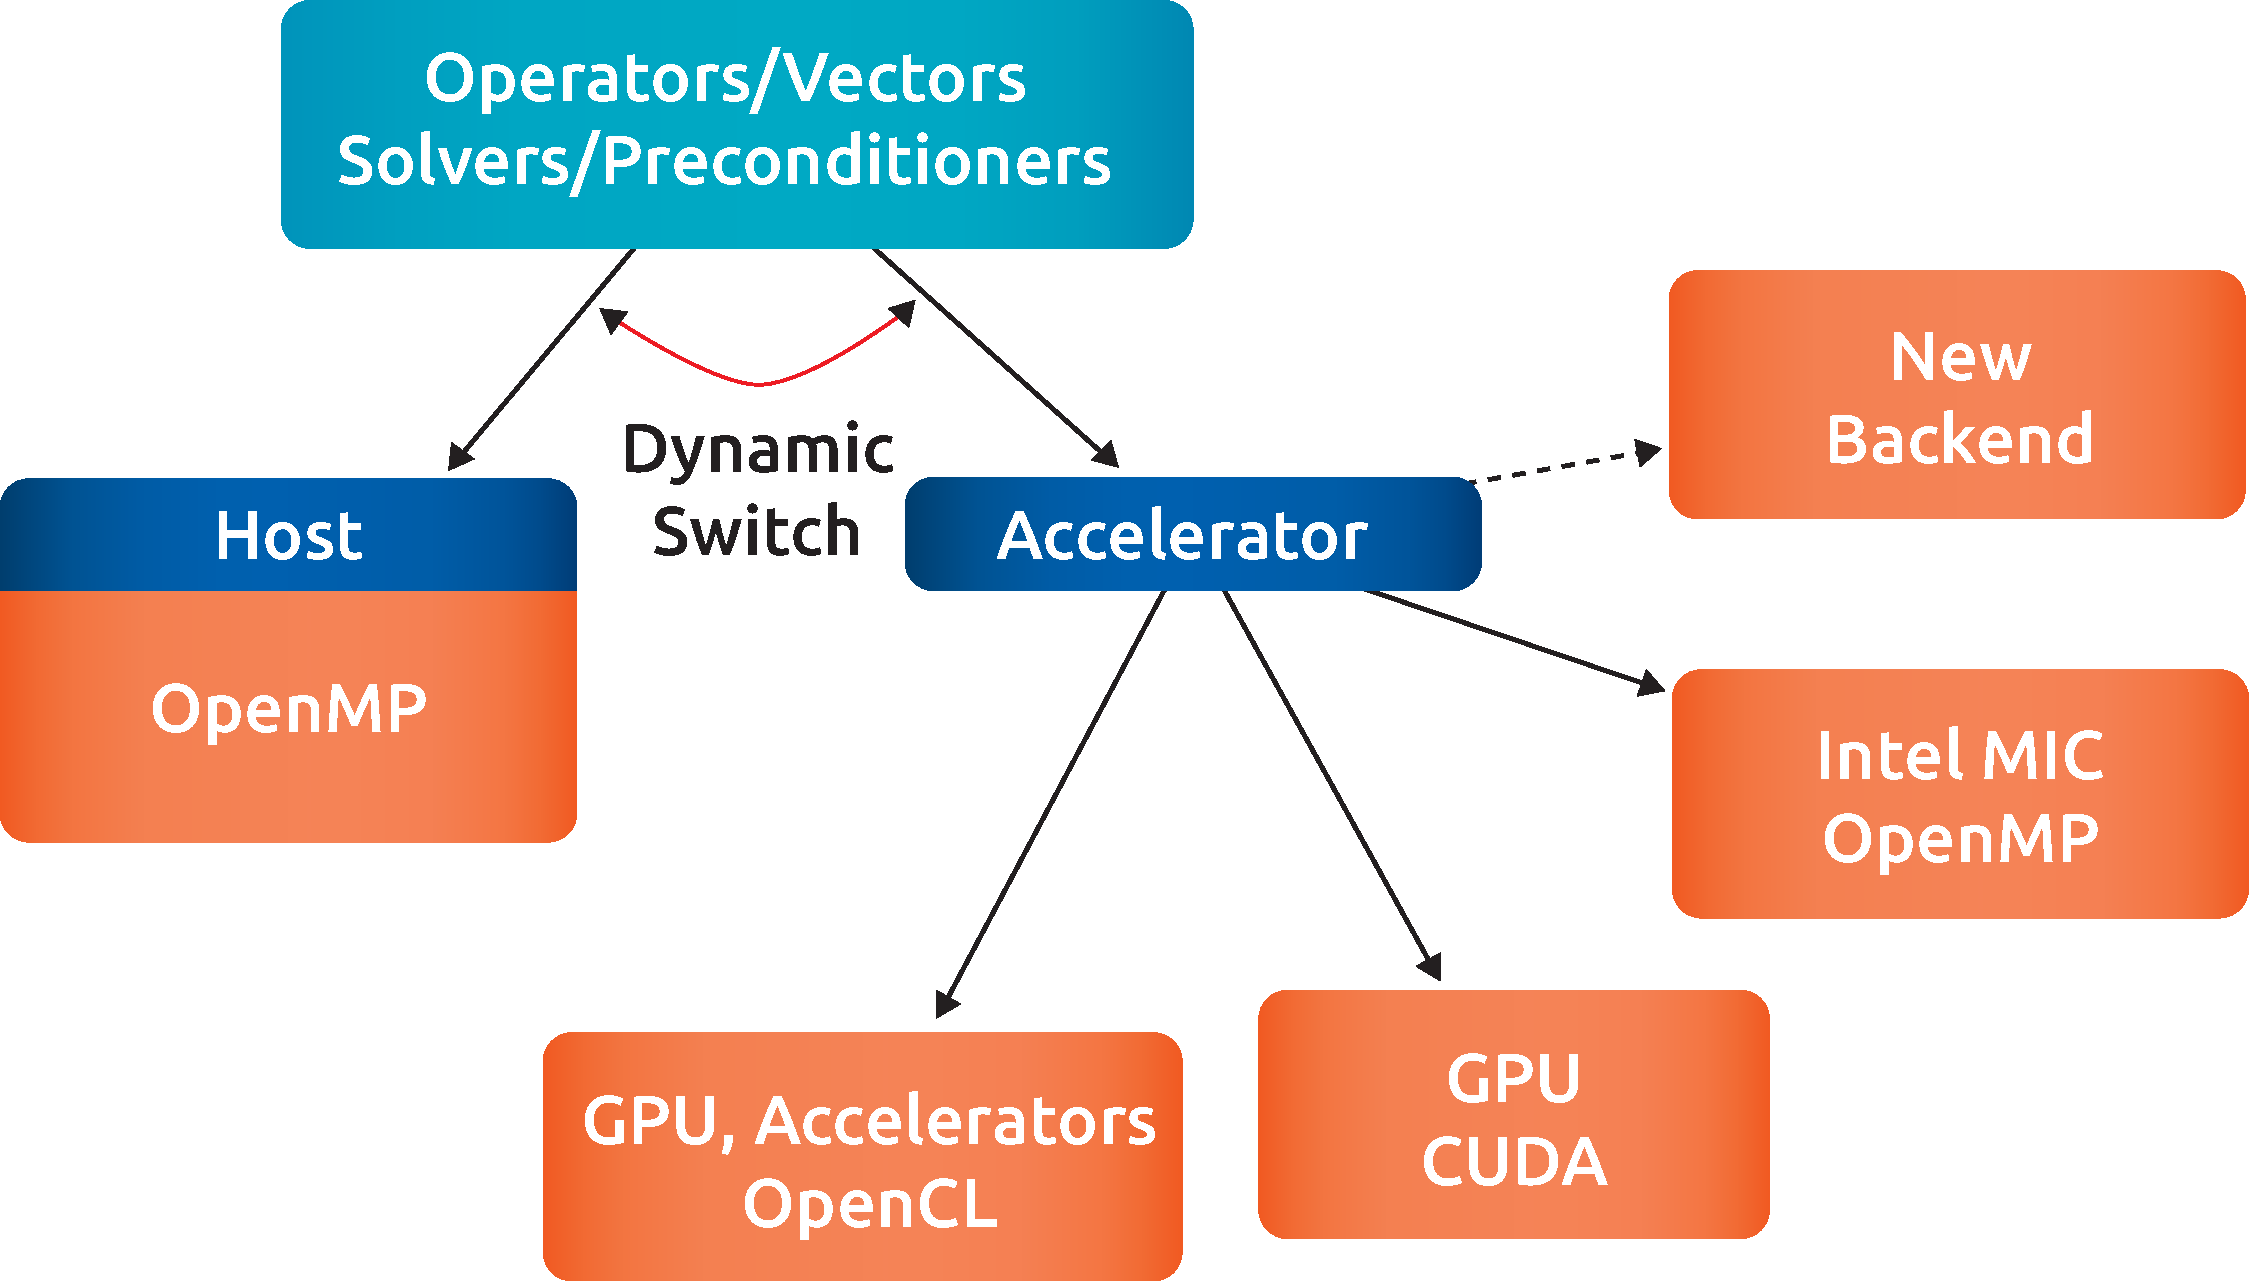
\includegraphics[width=0.6\textwidth]{./fig/structure.pdf}
\caption{Host and backends structure for different hardware}
\label{class-backends}
\end{figure}


The linear operators are defined as local or global matrices (i.e. on a single node or distributed/multi-node) and local stencils (i.e. matrix-free linear operations). 

\begin{figure}[!ht]
\centering
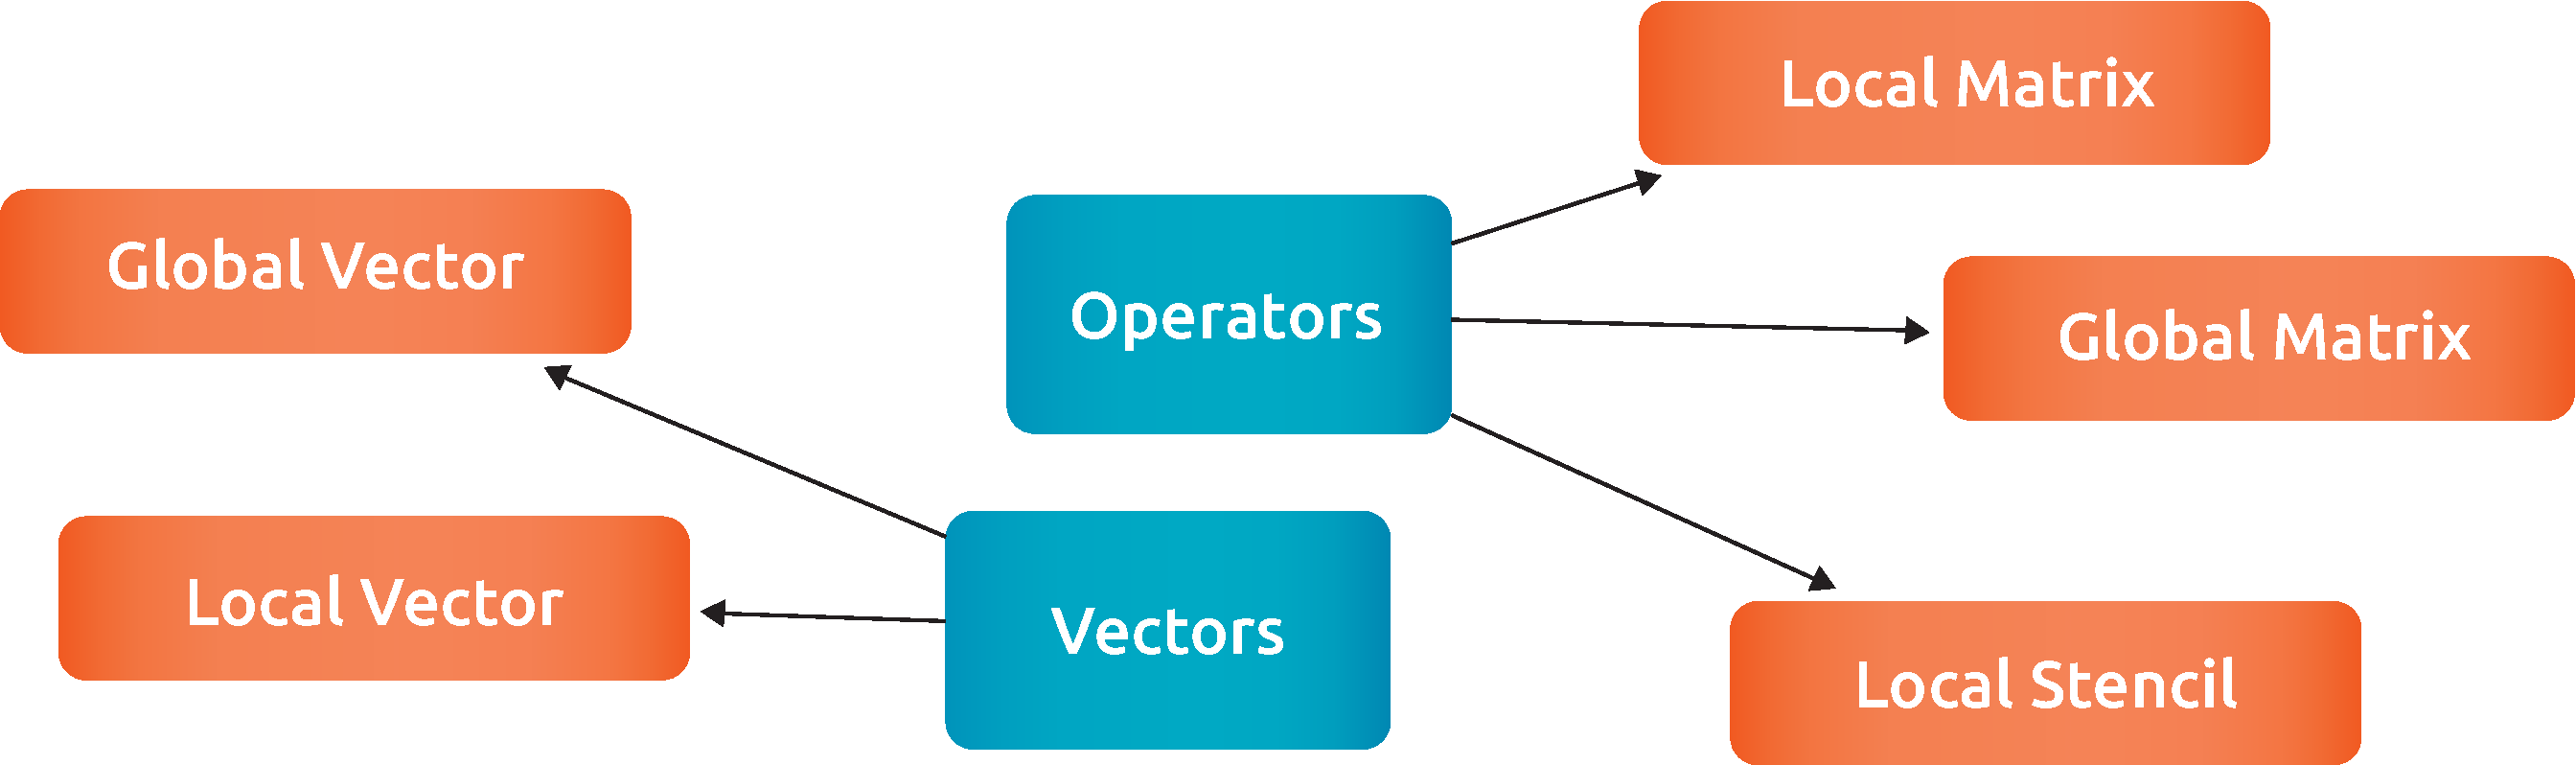
\includegraphics[width=0.85\textwidth]{./fig/operators.pdf}
\caption{Operator and vector classes}
\label{paralution-lib}
\end{figure}


The only template parameter of the operators and vectors is the data type (\emph{ValueType}). The operator data type could be \emph{float} or \emph{double}, while the vector data type can be \emph{float}, \emph{double} or \emph{int} (\emph{int} is used mainly for the permutation vectors). In the current version, cross ValueType object operations are not supported.


Each of the objects contain a local copy of the hardware descriptor created by the \emph{init\_platform()} function. This allows the user to modify it according to his needs and to obtain two or more objects with different hardware specifications (e.g. different amount of OpenMP threads, CUDA block sizes, etc).

\subsection{Local Operators/Vectors}

By Local Operators/Vectors we refer to Local Matrices and Stencils, and to Local Vectors. By \emph{Local} we mean the fact they stay on a single system. The system can contain several CPUs via UMA or NUMA memory system, it can contain an accelerator. 

\subsection{Global Operators/Vectors}

By Global Operators/Vectors we refer to Global Matrices and to Global Vectors. By \emph{Global} we mean the fact they can stay on a single or multiple nodes in a network. For this this type of computation, the communication is based on MPI.

\section{Functionality on the Accelerators}

Naturally, not all routines and algorithms can be performed efficiently on many-core systems (i.e. on accelerators). To provide full functionality the library has internal mechanisms to check if a particular routine is implemented on the accelerator. If not the object is moved to the host and the routine is computed there. This guarantees that your code will run (maybe not in the most efficient way) with any accelerator regardless of the available functionality for it.


